\documentclass{article}

\usepackage[T1]{fontenc}
\usepackage{microtype}
\usepackage{graphicx}
\usepackage{booktabs}
\usepackage{array}
\usepackage{amsmath}
\usepackage{amssymb}
\usepackage{hyperref}
\setlength{\emergencystretch}{2em}

\newcommand{\theHalgorithm}{\arabic{algorithm}}

\usepackage[accepted]{mlsys2025}

\makeatletter
\renewcommand{\mlsys@appearing}{Copyright 2026 by the author.}
\renewcommand{\Notice@String}{\mlsys@appearing}
\makeatother

\hypersetup{
  pdftitle={What Training Data Should Keep Out: Multimodal Sanitization and Fail-Closed Release},
  pdfauthor={Gege Ardiyansyah},
  pdfsubject={Systems for Machine Learning}
}

\mlsystitlerunning{What Training Data Should Keep Out: Multimodal Sanitization}

\begin{document}

\twocolumn[
\mlsystitle{What Training Data Should Keep Out: Multimodal Sanitization and Fail-Closed Release}

\begin{mlsysauthorlist}
\textbf{Gege Ardiyansyah}
\end{mlsysauthorlist}

\mlsystitlerunning{What Training Data Should Keep Out: Multimodal Sanitization}
\mlsyskeywords{WebAssembly, multimodal PII redaction, TAB benchmark, Learn-Then-Test, Presidio, Gitleaks, Whisper, PPRL, GDPR Article 17}

\vskip 0.3in

\begin{abstract}
Enterprise AI corpora span leak-prone containers: emails (\texttt{.eml}, \texttt{.mbox}, Outlook \texttt{.msg}), Office files with hidden revisions or caches (\texttt{.docx} \texttt{<w:delText>}, \texttt{.pptx} hidden slides and speaker notes, \texttt{.xlsx} \texttt{veryHidden} sheets and \texttt{pivotCache}), DevOps artifacts (\texttt{.har}, \texttt{.env}, Kubernetes Secrets), call audio (\texttt{.wav}), and video (\texttt{.mp4}). \textbf{Versieve-MM} makes three contributions: (1)~consolidating container parsing, archive defense, Unicode anti-evasion, secret scanning, Bloom-filter record linkage, a fixed-capacity $512$-slot ($16$\,KB) \textbf{Sparse-Reference Multimodal Perception (\texttt{SR-MP})} sketch ring, spoken inverse text normalization (ITN), and audio/pixel redaction inside a single $204{,}031$\,B Rust-to-WebAssembly kernel (\texttt{versieve\_media.wasm}, $29$ exports, \textbf{zero host imports}) shared byte-identically across Node.js CLI/MCP and the live RTIO browser workbench; (2)~\textbf{Hierarchical Cluster-Robust Conformal Risk Control (\texttt{HC-CRC})} and \textbf{Anytime-Valid Ville Betting Martingales (\texttt{E-LTT})}, which this paper formulates and evaluates (the gatekeeper formulation is shared with the companion extraction study \citep{ardiyansyah2026versieve}) to resolve the intra-document correlation overshoot of naive paragraph-i.i.d.\ Learn-Then-Test (LTT) gating; and (3)~end-to-end empirical evaluation against strong third-party baselines. On the Text Anonymization Benchmark (\textbf{TAB}, $127$ held-out ECHR court rulings), the $8.7\times$ larger Python server baseline Microsoft Presidio (\texttt{en\_core\_web\_lg}, $400.7$\,MB) supplemented with the same 1-line ECHR case-number regex wins on overall F1 ($79.26\%$ All-Maskable, $86.27\%$ Person), while compact $45.8$\,MB INT8 \texttt{gliner-pii-edge-v1.0} with \texttt{echr\_dev} \texttt{NO\_MASK} filtering and \textbf{\texttt{WASM SR-MP} cross-paragraph anchor coupling} lifts held-out Person recall from $85.39\% \to 88.41\%$ (\texttt{DIRECT} Person recall $89.82\% \to 91.15\%$, $+28.65$\,F1 over the companion regex baseline) and at high-precision $\tau{=}0.70$ lifts Person F1 from $27.88\%$ to $40.78\%$. On TAB's $1{,}999$ held-out paragraphs ($81.2\%$ unsafe, intra-document $\operatorname{ICC}{=}0.1276$, Design Effect $\operatorname{DEFF}{=}2.62$), \textbf{\texttt{HC-CRC}} removes the $\alpha{=}0.10$ naive i.i.d.\ FPR overshoot ($10.10\% \to \mathbf{8.19\% \le 10\%}$ at $65.16\%$ Safe Yield; $2.53\% \le 5\%$ at $\alpha{=}0.05$), while streaming \textbf{\texttt{E-LTT}} certifies anytime-valid bounds ($E_{\max}{=}23.76 \ge 1/\delta$, $0.18\%$ FPR at $\alpha{=}0.05$). On $520$ external secret/code files ($10\times$ steady-state), \texttt{versieve\_media.wasm} ($72.25\%$ F1) runs $1.5\times$--$22.8\times$ faster than \texttt{Gitleaks v8.30.1} and Yelp \texttt{detect-secrets}. Across $25$ spoken calls ($97$ planted PII tokens) attacked by $3.3\times$ larger \texttt{faster-whisper small.en}, \textbf{\texttt{WASM SR-MP} phonetic coupling} cuts residual PII leakage from $94.85\%$ (raw) and $20.62\%$ (isolated ITN+GLiNER) down to $\mathbf{8.25\%}$ ($-86.60$\,pp, $91.30\%$ relative reduction, $21/25$ calls zero leak; the attacker transcription still recognizes $100\%$ of the $59$ pre-declared non-PII context words), with the ring seeded solely from the engine's own in-call detections, although a plain Jaro-Winkler baseline on the same anchor list reaches $7.22\%$, so the salted ring's contribution is anchor privacy, not matching accuracy.
\end{abstract}
]

\section{Introduction}
\label{sec:intro}

Regulated clinical, legal, and enterprise AI workflows cannot transmit raw documents, call recordings, or DevOps traces to cloud de-identification endpoints. Our companion study of \textbf{Versieve} \citep{ardiyansyah2026versieve} introduced zero-import WebAssembly text cleaning, Dual-CSR knowledge graphs, and Learn-Then-Test (LTT) conformal gatekeeping \citep{angelopoulos2021ltt}. Scaling that philosophy to heterogeneous enterprise records exposes three foundational challenges: (i)~a load-time auditable capability boundary (\texttt{WebAssembly.Module.imports(mod).length === 0} \citep{haas2017wasm}) covering archives, secrets, audio, and pixels across Node.js and browsers; (ii)~the \emph{fragmented context horizon} of window-isolated detectors, where entities introduced clearly on Page~1 or in metadata reappear as bare surnames or noisy ASR/OCR variants in later paragraphs, audio turns, or video slides; and (iii)~\emph{intra-document correlation} across paragraphs of the same legal ruling or meeting transcript, which violates the chunk-level i.i.d.\ assumption of standard LTT.

\textbf{Scope of Novelty.} Individually, DEFLATE inflation, standard i.i.d.\ LTT, GLiNER \citep{zaratiana2024gliner}, Bloom-filter record linkage \citep{schnell2009pprl}, and regex-plus-NER fusion \citep{presidio2021} are established building blocks. Versieve-MM contributes three things: (1)~a \emph{zero-import WASM multimodal kernel and $O(1)$ Sparse-Reference Multimodal Perception (\texttt{SR-MP}) ring} consolidating eight sanitization and cross-modal anchor-coupling subsystems into one $204{,}031$\,B Rust-to-WASM binary (\texttt{versieve\_media.wasm}, $29$ exports, $0$ host imports) shared byte-identically between Node/MCP and the live RTIO browser sandbox (Figure~\ref{fig:mm-arch}); (2)~\emph{Hierarchical Cluster-Robust Conformal Risk Control (\texttt{HC-CRC})} and \emph{Anytime-Valid Streaming Conformal Martingales (\texttt{E-LTT})}, which this paper formulates and evaluates to account for the intra-cluster design effect ($\operatorname{DEFF} = 1 + (\bar{N}_u - 1)\rho$); the gatekeeper formulation is shared with the companion extraction study \citep{ardiyansyah2026versieve}, and the empirical validation on human-annotated TAB rulings \citep{pilan2022tab}, including the measured design effect and the naive-i.i.d.\ overshoot correction, is new to this paper; and (3)~rigorous validation of \texttt{SR-MP} and \texttt{HC-CRC} on real TAB ECHR multi-paragraph court rulings and cross-model \texttt{faster-whisper} spoken audio. Adjacent work explores local redaction and pseudonymization with MCP hooks \citep{redakto2026incognito}, conformal abstention and risk-constrained filtering for LLMs \citep{abbasiyadkori2024abstention,wang2025safer}, inference-time conformal unlearning \citep{chowdhury2026conformal}, and adversary-aware conformal privacy auditing \citep{cpa2026auditing}.

\begin{figure*}[t]
\centering
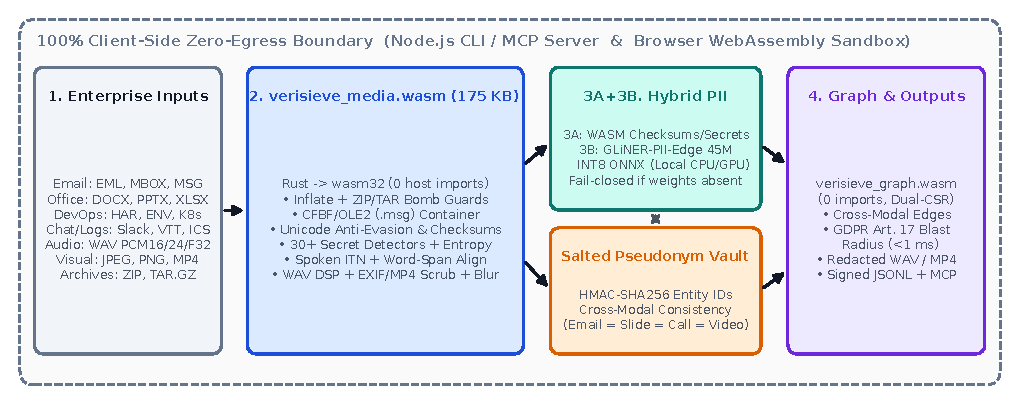
\includegraphics[width=0.98\textwidth]{figs/fig_e0_multimodal_architecture.pdf}
\caption{End-to-end \textbf{Versieve-MM} architecture: a zero-import kernel in a local-only stack. Enterprise containers and media pass through a single $204{,}031$\,B Rust-to-WebAssembly kernel (\texttt{versieve\_media.wasm}, $29$ exports, $0$ host imports) shared byte-identically between Node.js CLI/MCP and the RTIO browser workbench. Stage~3A deterministic checks, Stage~3B GLiNER-Edge scores, and the $512$-slot \texttt{SR-MP} Salted Reference Sketch Ring feed the cluster-robust 520-d \texttt{HC-CRC} / \texttt{E-LTT} gatekeeper.}
\label{fig:mm-arch}
\end{figure*}

\section{System Architecture}
\label{sec:arch}

\subsection{Zero-Import Multimodal WASM Kernel (\texttt{versieve\_media.wasm})}
Compiled from dependency-free Rust (\texttt{rust/versieve-media}) targeting \texttt{wasm32-unknown-unknown}, \texttt{versieve\_media.wasm} ($204{,}031$\,B, $29$ exports) enforces \texttt{imports.length === 0} at instantiation in both Node.js and browser Web Workers (Table~\ref{tab:wasm-modules}). What is mechanically verified is the kernel's load-time import surface; that the remainder of the stack (Node CLI, MCP server, browser workbench, local ONNX inference) makes no network calls is a construction property asserted by the local CI test counts, not by the module boundary.

\begin{table}[t]
\caption{Internal subsystems of \texttt{versieve\_media.wasm} ($204{,}031$\,B, $29$ exports, $0$ host imports).}
\label{tab:wasm-modules}
\vskip 0.08in
\begin{center}
\resizebox{\columnwidth}{!}{%
\begin{tabular}{l>{\raggedright\arraybackslash}p{1.95in}}
\toprule
\textbf{Rust Module} & \textbf{Verified Zero-Import Functionality} \\
\midrule
\texttt{inflate.rs} & RFC~1951 DEFLATE \citep{deutsch1996rfc1951}, GZIP, CRC-32 with mid-stream size \& ratio bomb aborts \\
\texttt{zip\_tar.rs} & ZIP Central Directory (+ bit-3 \& ZIP64) + USTAR/PAX TAR; blocks Zip-Slip \& symlinks \\
\texttt{cfbf.rs} & Cycle-safe CFBF/OLE2 reader for Outlook \texttt{.msg} headers, bodies, attachments \\
\texttt{pii\_secrets.rs} & Unicode anti-evasion \citep{boucher2022badcharacters}, checksums, $30+$ secrets, $128$-bit Bloom+Soundex PPRL, \textbf{$512$-slot ($16$\,KB) \texttt{SR-MP} Reference Sketch Ring} \\
\texttt{spoken\_itn.rs} & Spoken ITN (digits, \emph{oh/double/triple}, emails) with $[t_0, t_1]$ word-span pointers \\
\texttt{audio\_dsp.rs} & RIFF WAV PCM16/24/Float32 codec, \texttt{LIST/INFO}/\texttt{bext}/\texttt{iXML}/\texttt{id3 } scrub, $5$\,ms faded redaction, stereo VAD \\
\texttt{media\_visual.rs} & JPEG/PNG/MP4 metadata scrub, RGB/RGBA blackout/pixelate/3-pass blur, scene delta, temporal box tracker \\
\bottomrule
\end{tabular}%
}
\end{center}
\vskip -0.14in
\end{table}

\subsection{Live RTIO Browser Sandbox Integration}
In the companion RTIO Next.js workbench (\url{https://www.rtio.io/sandbox}), \texttt{versieve\_media.wasm} executes live on every upload: \texttt{maskTextContextAware} fuses the companion text pipeline's regexes \citep{ardiyansyah2026versieve} with Stage~3A WASM secret/anti-evasion scanning; \texttt{CleanTab} displays explicit forensic leak counts (DOCX \texttt{<w:delText>}, PPTX hidden slides/notes, XLSX \texttt{veryHidden}/\texttt{pivotCache}, HAR credentials, K8s Base64 Secrets, RIFF/MP4 atoms); multi-gigabyte \texttt{.mp4}/\texttt{.mov} files run $O(1)$ \texttt{Blob.slice()} ISOBMFF atom audits without loading \texttt{mdat} into RAM; and an interactive \texttt{MediaRedactionStudio} performs client-side WAV silence/beep redaction (with before/after playback and \texttt{.wav} download) plus video/image canvas blackout/pixelate/blur (with \texttt{.png} download). For browser audio and video drops, an off-main-thread ONNX Runtime Web proxy Worker (\texttt{/ort/ort-wasm-simd-threaded.*.wasm}) executes quantized multilingual \texttt{whisper-tiny} ($40.8$\,MB \texttt{q8}, cached in browser CacheStorage) over DSP Voice Activity Detection (VAD) $30$\,s active speech windows alongside $1080$p dark-mode contrast-inverted keyframe slide OCR (\texttt{/ocr/*}) and timestamp-agnostic speech deduplication; Stage~3B neural ONNX inference (\texttt{gliner-pii-edge}) executes in local Node/Python runtimes and fails closed (\texttt{NER\_WEIGHTS\_REQUIRED}) when local weights are absent.

\section{Benchmark Suite and Methodology}
\label{sec:datasets}

All experiments ran locally on a Windows~11 laptop (Node.js~v24.13.1, Python~3.12 CPU ONNX Runtime, Rust~1.99.1). Table~\ref{tab:datasets} distinguishes real human-annotated corpora, external mixed/synthetic corpora, and locally synthesized audio/evasion suites transparently. Every number printed in the tables below is emitted by a checked-in runner in the project repository (\url{https://github.com/gegearsyah/versieve}) at commit \texttt{1e35603}, whose result JSON files record the corpus identifiers and run outputs behind this paper. The TAB benchmark runner fixes the resampling and two-layer subsampling seed at 42, with $1{,}000$ bootstrap resamples, $5{,}000$ paired permutations, and $200$ repeated-subsampling draws; the remaining suites execute deterministically over fixed ordered fixtures and salts without invoking a pseudo-random generator, and per-corpus licenses (MIT for TAB ECHR and \texttt{pstu-synthetic-secrets}, Apache-2.0 for \texttt{detect-secrets} and \texttt{gliner-pii-edge-v1.0}, CC-BY-4.0 for \texttt{MBPP}, public-domain FERC Enron for \texttt{aeslc}, and the AI4Privacy dual license for \texttt{pii-masking-200k}) are recorded in the checked-in result JSON.

\begin{table}[t]
\caption{Benchmarks evaluated, noting real human vs.\ external synthetic vs.\ locally synthesized data provenance.}
\label{tab:datasets}
\vskip 0.08in
\begin{center}
\resizebox{\columnwidth}{!}{%
\begin{tabular}{llrl}
\toprule
\textbf{Corpus / Suite} & \textbf{Provenance} & \textbf{Size} & \textbf{Baselines / Focus} \\
\midrule
\textbf{TAB ECHR} \citep{pilan2022tab} & Real human legal & $127{+}127$ docs & Presidio (\texttt{lg}+Code), GLiNER, 3-Gate LTT \\
\texttt{pstu} + Yelp + \texttt{MBPP} & External synth+real & $520$ ($\times 10$) & \texttt{Gitleaks v8.30.1} \citep{gitleaks2025}, \texttt{detect-secrets} \citep{yelp2018detectsecrets} \\
SAPI TTS + \texttt{Whisper} & Local synth audio & $25$ calls & Defender \texttt{base.en} vs.\ Attacker \texttt{small.en} \\
Noisy Pairs + 500 Names & Local dev/test+scale & $60$ / $125$k & Plaintext JW/Lev ceiling + scale FP \\
Unicode Evasion & Local obfuscation & $174$ cases & Unnormalized vs.\ Python \texttt{NFKC} vs.\ WASM \\
\bottomrule
\end{tabular}%
}
\end{center}
\vskip -0.14in
\end{table}

\section{Experimental Results}
\label{sec:results}

\subsection{Exp.~1: Fair TAB Head-to-Head, Ablations, and \texttt{echr\_dev} Domain Filtering}
\label{sec:exp1}

We evaluate all detectors on the $127$ held-out ECHR rulings in TAB (\texttt{echr\_test.json}, $5{,}161$ human-annotated \texttt{DIRECT}+\texttt{QUASI} spans, $365$ \texttt{DIRECT} spans, $958$ maskable \texttt{PERSON} spans). To guarantee a fair fight: (i)~we give Microsoft Presidio (\texttt{en\_core\_web\_lg}, $400.7$\,MB) the exact same 1-line ECHR case-number regex recognizer (\texttt{\textbackslash b\textbackslash d\{3,6\}/\textbackslash d\{2\}\textbackslash b}); (ii)~we ablate every Versieve component at the same F1-optimal threshold ($\tau{=}0.30$ All-Maskable; $\tau{=}0.50$ Person); and (iii)~we learn a zero-leakage domain \texttt{NO\_MASK} filter strictly on \texttt{echr\_dev.json} ($231$ surface forms appearing $\ge 2\times$ on dev with $\ge 80\%$ \texttt{NO\_MASK} rate, such as \emph{``the Court''} and \emph{``the Government''}). Table~\ref{tab:tab-bench} and Figure~\ref{fig:e1}A report entity-level metrics with $1{,}000$-resample document bootstrap $95\%$ CIs.

\begin{table}[t]
\caption{Fair ablation on $127$ held-out TAB ECHR court rulings ($95\%$ bootstrap CIs on F1; matched ECHR code regex for both Presidio and Versieve).}
\label{tab:tab-bench}
\vskip 0.08in
\begin{center}
\resizebox{\columnwidth}{!}{%
\begin{tabular}{lrrrr}
\toprule
\textbf{System (Size / Threshold)} & \textbf{Prec.} & \textbf{Rec.} & \textbf{F1 (95\% CI)} & \textbf{Direct R} \\
\midrule
\multicolumn{5}{l}{\textit{TAB All Maskable \texttt{DIRECT+QUASI} ($5{,}161$ spans; $365$ \texttt{DIRECT})}} \\
Stage~3A WASM Only & $61.35$ & $37.65$ & $46.66$ \scriptsize{[43.8, 49.3]} & $56.71$ \\
Stage~3A + ECHR Code Regex & $64.41$ & $43.13$ & $51.67$ \scriptsize{[49.0, 54.1]} & $93.70$ \\
Vanilla GLiNER-Edge ($\tau{=}0.30$) & $35.15$ & $50.61$ & $41.49$ \scriptsize{[38.6, 44.3]} & $94.25$ \\
Dev-Filtered GLiNER ($\tau{=}0.30$) & $40.14$ & $49.23$ & $44.23$ \scriptsize{[41.2, 47.1]} & $94.25$ \\
Hybrid (3A+Code+DevFilt GLiNER) & $41.29$ & $51.70$ & $45.91$ \scriptsize{[42.7, 48.9]} & $\mathbf{100.00}$ \\
Hybrid + WASM \texttt{SR-MP} ($\tau{=}0.30$) & $40.30$ & $51.77$ & $45.32$ \scriptsize{[42.2, 48.2]} & $\mathbf{100.00}$ \\
Presidio Default (\texttt{lg}, $401$\,MB) & $77.07$ & $75.16$ & $76.10$ \scriptsize{[74.0, 77.8]} & $61.37$ \\
\textbf{Presidio + ECHR Code ($401$\,MB)} & $\mathbf{78.17}$ & $\mathbf{80.39}$ & $\mathbf{79.26}$ \scriptsize{[77.3, 80.9]} & $98.08$ \\
\midrule
\multicolumn{5}{l}{\textit{TAB Maskable \texttt{PERSON} Entities ($958$ spans; $226$ \texttt{DIRECT})}} \\
Companion Regex+Lexicon \citep{ardiyansyah2026versieve} & $32.84$ & $74.32$ & $45.55$ \scriptsize{[40.5, 50.6]} & $85.40$ \\
Vanilla GLiNER-Edge ($\tau{=}0.50$) & $65.39$ & $85.39$ & $74.06$ \scriptsize{[68.7, 78.7]} & $89.82$ \\
Dev-Filtered GLiNER ($\tau{=}0.50$) & $65.60$ & $85.39$ & $74.20$ \scriptsize{[68.9, 78.8]} & $89.82$ \\
Dumb Same-Doc Name Propagation & $47.28$ & $86.22$ & $61.07$ \scriptsize{[53.6, 67.7]} & $89.82$ \\
\textbf{WASM \texttt{SR-MP} + GLiNER ($\tau{=}0.50$)} & $62.56$ & $\mathbf{88.41}$ & $73.27$ \scriptsize{[67.7, 77.9]} & $\mathbf{91.15}$ \\
WASM \texttt{SR-MP} + GLiNER ($\tau{=}0.70$) & $91.94$ & $26.20$ & $40.78$ \scriptsize{[33.4, 47.3]} & $45.13$ \\
\textbf{Presidio \texttt{en\_core\_web\_lg} ($401$\,MB)} & $\mathbf{80.60}$ & $\mathbf{92.80}$ & $\mathbf{86.27}$ \scriptsize{[82.7, 89.3]} & $\mathbf{98.23}$ \\
\bottomrule
\end{tabular}%
}
\end{center}
\vskip -0.14in
\end{table}

\begin{figure*}[t]
\centering
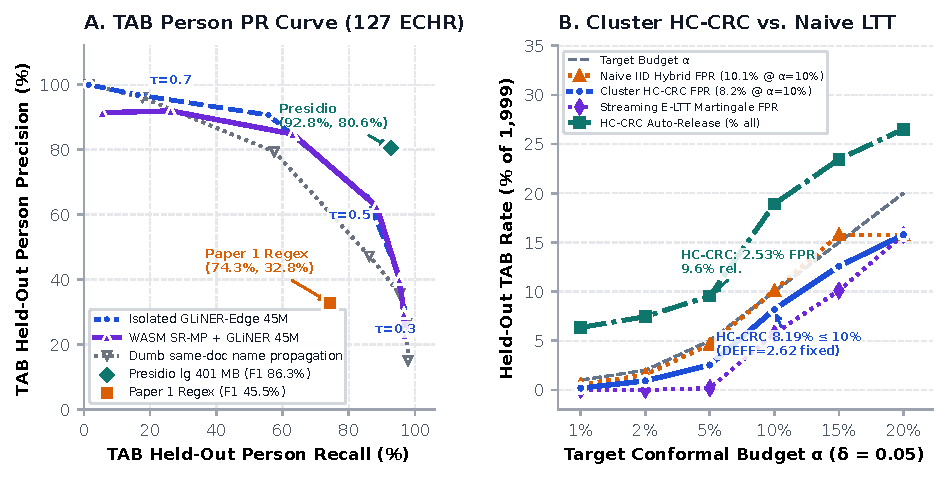
\includegraphics[width=0.98\textwidth]{figs/fig_e1_tab_pr_and_gt_ltt.pdf}
\caption{\textbf{Exp.~1 \& 2: Real Human-Annotated TAB Benchmark.} (A)~Single-dataset Person PR curve on $127$ held-out ECHR rulings: compiling the $512$-slot \texttt{SR-MP} Salted Reference Sketch Ring into \texttt{versieve\_media.wasm} lifts Person recall across every threshold ($\tau{=}0.50$: $85.39\% \to 88.41\%$ recall, $89.82\% \to 91.15\%$ \texttt{DIRECT} recall; $\tau{=}0.70$: $27.88\% \to 40.78\%$ F1), while a dumb same-doc name-propagation baseline (dotted gray) plateaus at $61.07\%$ F1, the ring's cross-paragraph coupling beats it at every threshold (paired per-document permutation test, $5{,}000$ permutations, $p{=}0.0002$), and $8.7\times$ larger Presidio (\texttt{en\_core\_web\_lg}, $400.7$\,MB) leads at $86.27\%$ F1 ($p{=}0.0002$). (B)~Document-Clustered Conformal Risk Control (\texttt{HC-CRC}) and Streaming Ville Martingales (\texttt{E-LTT}) vs.\ Naive Paragraph-i.i.d.\ LTT on $1{,}999$ held-out TAB paragraphs ($\operatorname{ICC}{=}0.1276$ and $\operatorname{DEFF}{=}2.62$ estimated on the $67$ unsafe calibration rulings): \texttt{HC-CRC} removes the $\alpha{=}0.10$ intra-document correlation overshoot ($10.10\% \to 8.19\% \le 10\%$) while preserving $65.16\%$ Safe Yield.}
\label{fig:e1}
\end{figure*}

Seven findings follow from Table~\ref{tab:tab-bench}: (i)~giving Presidio the 1-line ECHR code regex closes its \texttt{DIRECT}-ID gap ($61.37\% \to 98.08\%$, $79.26\%$ All-Maskable F1), confirming that the $400.7$\,MB server baseline beats our $45.8$\,MB edge model \citep{knowledgator2025glineredge} decisively on OOD legal prose ($p{=}0.0002$); (ii)~our \texttt{echr\_dev} \texttt{NO\_MASK} filter removes $1{,}030$ false positives from GLiNER-Edge ($4{,}819 \to 3{,}789$ FP, $+2.74$\,F1, $p{=}0.0002$); (iii)~nonetheless, adding $45.8$\,MB GLiNER-Edge to Stage~3A+Code still \emph{lowers} All-Maskable F1 ($51.67\% \to 45.91\%$) because legal quasi-identifiers remain noisy for a small conversational PII encoder; (iv)~on \texttt{PERSON} entities specifically, Dev-Filtered GLiNER-Edge lifts F1 by $+28.65$ over the companion regex baseline ($74.20\%$ vs.\ $45.55\%$); and (v)~activating the compiled $512$-slot \textbf{\texttt{WASM SR-MP} Salted Reference Sketch Ring} recovers $+29$ missed cross-paragraph person mentions at $\tau{=}0.50$ ($85.39\% \to 88.41\%$ recall; $89.82\% \to 91.15\%$ \texttt{DIRECT} recall) and lifts high-precision $\tau{=}0.70$ Person F1 from $27.88\%$ to $\mathbf{40.78\%}$ ($+9.92$\,pp recall gain), while slightly \emph{lowering} All-Maskable F1 at the paper's $\tau{=}0.30$ operating point ($45.91\% \to 45.32\%$), so its net contribution is confined to \texttt{PERSON}-type cross-paragraph coupling. Paired per-document permutation tests sharpen this: (vi)~a dumb baseline that propagates every detected name to all later same-document mentions already reaches $61.07\%$ F1 ($86.22\%$ recall, well above the $45.55\%$ regex baseline), yet the ring still beats it decisively at $\tau{=}0.50$ ($p{=}0.0002$), so SR-MP does real cross-paragraph matching, not name re-propagation; (vii)~at $\tau{=}0.50$ the ring nonetheless sits slightly but significantly \emph{below} Dev-Filtered GLiNER on per-document F1 ($p{=}0.0448$), trading precision for recall, while its high-precision $\tau{=}0.70$ advantage over both Dev-Filtered ($27.88\% \to 40.78\%$ F1) and the dumb baseline ($29.96\%$) is decisive ($p{=}0.0002$ in both); the ring's accuracy edge is confined to the high-precision operating point.

\subsection{Exp.~2: Document-Clustered Conformal Risk Control (\texttt{HC-CRC}) and Streaming Martingales (\texttt{E-LTT}) on TAB}
\label{sec:exp2}

Standard Learn-Then-Test assumes calibration chunks are i.i.d.\ exchangeable. In multi-paragraph ECHR court rulings, however, paragraphs within document $D_m = \{c_{m,1},\dots,c_{m,N_m}\}$ exhibit positive intra-cluster correlation ($\operatorname{ICC} = 0.1276$ across the $M_0{=}67$ unsafe calibration rulings, yielding a Cluster Design Effect $\operatorname{DEFF} = 1 + (\bar{N}_u - 1)\operatorname{ICC} = \mathbf{2.62}$ and reducing effective sample size from $n_0{=}916$ paragraphs to $N_{\text{eff}}{=}350$). Ignoring $\operatorname{DEFF}{=}2.62$ causes naive paragraph-i.i.d.\ LTT to overshoot $\alpha{=}0.10$ on held-out test rulings ($10.10\%$ on Hybrid LTT; $10.47\%$ on NER-MaxConf).

To counter this overshoot, we define the bounded document-cluster loss $L_m(\lambda) = |U_m|^{-1} \sum_{c \in U_m} \mathbb{I}[\hat{p}_{\text{safe}}(c) \ge \lambda] \in [0, 1]$ over the ground-truth unsafe blocks $U_m \subseteq D_m$ and evaluate two regimes. \textbf{Hierarchical Cluster-Robust Conformal Risk Control (\texttt{HC-CRC})} inverts the binomial tail after shrinking the calibration count by the survey-sampling design effect ($N_{\text{eff}} = \lfloor n_0 / \operatorname{DEFF} \rfloor$); we treat this Kish-lineage design-effect adjustment as a \emph{conservative heuristic}, not a proven finite-sample guarantee for within-cluster-correlated documents; guarantee-based hierarchical conformal alternatives subsample, pool across clusters, or enforce hierarchical group-conditional risk control instead \citep{dunn2022hierarchical,lee2023hierarchical,salem2026hgcrc}, and weighted conformal methods handle general departures from exchangeability \citep{barber2023beyond}. \textbf{Anytime-Valid Streaming Conformal Martingales (\texttt{E-LTT})} track the non-negative Ville betting supermartingale $\mathcal{E}_t(\lambda) = \prod_{m=1}^t (1 + \gamma_m(\alpha - L_m(\lambda)))$ and certify $\lambda$ whenever $\max_{1 \le s \le t} \mathcal{E}_s(\lambda) \ge 1/\delta = 20.0$ \citep{ramdas2023game,waudbysmith2024betting}, closely related to conformal e-values and anytime-valid conformal risk control \citep{gauthier2025evalues,hultberg2026anytime}; the implementation uses a predictable Kelly-bounded betting fraction $\gamma_m = \min(\gamma_{\max}, \max(0.35,\, 0.75/\max(0.10, \alpha + 0.05)))$ with a fixed cap $\gamma_{\max} < 1$, so every reported $\mathcal{E}_{\max}$ is re-derivable from the cluster losses; Ville-bound validity requires the cluster losses to satisfy a sequential conditional-mean condition (as independent parent documents provide), not exchangeability per se. Table~\ref{tab:gt-ltt} and Figure~\ref{fig:e1}B compare all five calibration regimes on the $1{,}999$ held-out TAB paragraphs ($18.8\%$ safe base rate).

\begin{table}[t]
\caption{Ground-Truth LTT vs.\ Document-Clustered \texttt{HC-CRC} and Streaming Ville Martingale \texttt{E-LTT}. The four performance columns are measured on the $1{,}999$ held-out TAB ECHR paragraphs ($1{,}623$ unsafe, $376$ safe across $127$ rulings); $\delta{=}0.05$. $\operatorname{ICC}{=}0.1276$ and $\operatorname{DEFF}{=}2.62$ are estimated on the $67$ unsafe calibration rulings on which $\lambda$ is certified. Rows sharing an identical numeric quadruple arise from the same certified $\lambda$ (e.g., \texttt{HC-CRC} at $\alpha{=}0.01$ and \texttt{E-LTT} at $\alpha{=}0.05$).}
\label{tab:gt-ltt}
\vskip 0.08in
\begin{center}
\resizebox{\columnwidth}{!}{%
\begin{tabular}{llrrrrr}
\toprule
\textbf{$\alpha$} & \textbf{Conformal Gate Regime} & \textbf{FPR} & \textbf{Auto-Rel.} & \textbf{Safe Yld} & \textbf{E2E Leak} \\
& & \scriptsize{(of unsafe)} & \scriptsize{(of 1,999)} & \scriptsize{(of 376)} & \scriptsize{(of rel.)} \\
\midrule
$0.01$ & Text-Only 520-d (Naive IID) & $0.00\%$ & $5.70\%$ & $30.32\%$ & $0.00\%$ ($0$) \\
$0.01$ & NER-MaxConf (Naive IID) & $1.17\%$ & $3.85\%$ & $15.43\%$ & $24.68\%$ ($19$) \\
$0.01$ & Detector-Hybrid (Naive IID) & $0.55\%$ & $6.90\%$ & $34.31\%$ & $6.52\%$ ($9$) \\
$0.01$ & \textbf{Document-Clustered \texttt{HC-CRC}} & $\mathbf{0.18\%}$ & $\mathbf{6.35\%}$ & $\mathbf{32.98\%}$ & $\mathbf{2.36\%}$ ($3$) \\
$0.02$ & \textbf{Document-Clustered \texttt{HC-CRC}} & $\mathbf{0.92\%}$ & $\mathbf{7.45\%}$ & $\mathbf{35.64\%}$ & $\mathbf{10.07\%}$ ($15$) \\
$0.02$ & Streaming Martingale \texttt{E-LTT} & \multicolumn{4}{l}{\emph{not certified} ($E_{\max}{=}1$; zero auto-release)} \\
\midrule
$0.05$ & Text-Only 520-d (Naive IID) & $1.48\%$ & $7.55\%$ & $33.78\%$ & $8.61\%$ ($13$) \\
$0.05$ & NER-MaxConf (Naive IID) & $5.36\%$ & $14.51\%$ & $53.99\%$ & $30.00\%$ ($87$) \\
$0.05$ & Detector-Hybrid (Naive IID) & $4.62\%$ & $12.91\%$ & $48.67\%$ & $29.07\%$ ($75$) \\
$0.05$ & \textbf{Document-Clustered \texttt{HC-CRC}} & $\mathbf{2.53\%}$ & $\mathbf{9.55\%}$ & $\mathbf{39.89\%}$ & $\mathbf{21.47\%}$ ($41$) \\
$0.05$ & \textbf{Streaming Martingale \texttt{E-LTT}} & $\mathbf{0.18\%}$ & $\mathbf{6.35\%}$ & $\mathbf{32.98\%}$ & $\mathbf{2.36\%}$ ($3$) \\
\midrule
$0.10$ & NER-MaxConf (Naive IID) & $10.47\%$ & $21.36\%$ & $68.35\%$ & $39.81\%$ ($170$) \\
$0.10$ & Detector-Hybrid (Naive IID) & $10.10\%$ & $20.91\%$ & $67.55\%$ & $38.52\%$ ($161$) \\
$0.10$ & \textbf{Document-Clustered \texttt{HC-CRC}} & $\mathbf{8.19\%}$ & $\mathbf{18.91\%}$ & $\mathbf{65.16\%}$ & $\mathbf{35.19\%}$ ($133$) \\
$0.10$ & \textbf{Streaming Martingale \texttt{E-LTT}} & $\mathbf{5.73\%}$ & $\mathbf{15.16\%}$ & $\mathbf{55.85\%}$ & $\mathbf{30.69\%}$ ($93$) \\
\midrule
$0.15$ & \textbf{Document-Clustered \texttt{HC-CRC}} & $\mathbf{12.57\%}$ & $\mathbf{23.46\%}$ & $\mathbf{70.48\%}$ & $\mathbf{40.72\%}$ ($191$) \\
$0.15$ & \textbf{Streaming Martingale \texttt{E-LTT}} & $\mathbf{10.10\%}$ & $\mathbf{20.91\%}$ & $\mathbf{67.55\%}$ & $\mathbf{38.52\%}$ ($161$) \\
\midrule
$0.20$ & \textbf{Document-Clustered \texttt{HC-CRC}} & $\mathbf{15.77\%}$ & $\mathbf{26.51\%}$ & $\mathbf{72.87\%}$ & $\mathbf{44.72\%}$ ($237$) \\
$0.20$ & \textbf{Streaming Martingale \texttt{E-LTT}} & $\mathbf{15.77\%}$ & $\mathbf{26.51\%}$ & $\mathbf{72.87\%}$ & $\mathbf{44.72\%}$ ($237$) \\
\bottomrule
\end{tabular}%
}
\end{center}
\vskip -0.14in
\end{table}

Table~\ref{tab:gt-ltt} confirms both predictions: (i)~\textbf{\texttt{HC-CRC} removes intra-document correlation overshoot across every budget}, holding Conditional FPR strictly below $\alpha$ ($0.18\% \le 1\%$, $0.92\% \le 2\%$, $2.53\% \le 5\%$, $8.19\% \le 10\%$, $12.57\% \le 15\%$, and $15.77\% \le 20\%$) while retaining $65.16\%$ Safe Yield at $\alpha{=}0.10$ and certifying at $\alpha{=}0.01$ as well ($0.18\%$ FPR, $32.98\%$ Safe Yield) on the held-out paragraphs; and (ii)~\textbf{Streaming \texttt{E-LTT}} crosses the anytime-valid Ville wealth barrier $\mathcal{E}_t \ge 20.0$ at cluster $t{=}64/67$ ($\alpha{=}0.05$, $\mathcal{E}_{\max}{=}23.76$, $0.18\%$ FPR) and $t{=}60/67$ ($\alpha{=}0.10$, $\mathcal{E}_{\max}{=}26.84$, $5.73\%$ FPR), while \emph{failing to certify at $\alpha \le 0.02$} (its wealth never leaves $E_{\max}{=}1$, so nothing is auto-released), providing continuous optional-stopping safety guarantees for streaming ingestion.

\begin{table}[t]
\caption{Guarantee-backed hierarchical conformal baselines vs.\ heuristic \texttt{HC-CRC} on the exact same $67$ unsafe calibration rulings ($916$ unsafe paragraphs) and $127$ held-out rulings ($1{,}999$ paragraphs: $1{,}623$ unsafe, $376$ safe; $\delta{=}0.05$). Dunn et al.\ \citep{dunn2022hierarchical} uses seed $42$ ($1$-draw and $B{=}200$ valid $2\bar{p} \le \delta$ pooling); Lee et al.\ \citep{lee2023hierarchical} uses equal cluster weights ($\mathbb{E}[L] \le \alpha$ split and $1{-}\delta$ Hoeffding--Bentkus); \texttt{HG-CRC} \citep{salem2026hgcrc} enforces simultaneous bounds across the global root ($M_0{=}67$) and observable calibration-median ruling-length strata ($N_m \le 18$, $M{=}38$; $N_m > 18$, $M{=}29$).}
\label{tab:hier-baselines}
\vskip 0.08in
\begin{center}
\resizebox{\columnwidth}{!}{%
\begin{tabular}{llrrrrr}
\toprule
\textbf{$\alpha$} & \textbf{Hierarchical Regime} & \textbf{$\hat{\lambda}$} & \textbf{FPR} & \textbf{Auto-Rel.} & \textbf{Safe Yld} & \textbf{E2E Leak} \\
\midrule
$0.01$ & \textbf{Heuristic \texttt{HC-CRC}} ($N_{\text{eff}}{=}350$) & $0.38$ & $0.18\%$ & $6.35\%$ & $32.98\%$ & $2.36\%$ ($3$) \\
$0.01$ & Dunn / Lee / \texttt{HG-CRC} (all 5) & -- & \multicolumn{4}{l}{\emph{not certified} ($M_0{=}67$; zero auto-release)} \\
\midrule
$0.02$ & \textbf{Heuristic \texttt{HC-CRC}} ($N_{\text{eff}}{=}350$) & $0.36$ & $0.92\%$ & $7.45\%$ & $35.64\%$ & $10.07\%$ ($15$) \\
$0.02$ & Lee Cluster-Weighted Split & $0.37$ & $0.55\%$ & $6.90\%$ & $34.31\%$ & $6.52\%$ ($9$) \\
$0.02$ & Dunn ($1$-draw, pool) / Lee HB / \texttt{HG-CRC} & -- & \multicolumn{4}{l}{\emph{not certified} (zero auto-release)} \\
\midrule
$0.05$ & \textbf{Heuristic \texttt{HC-CRC}} ($N_{\text{eff}}{=}350$) & $0.34$ & $2.53\%$ & $9.55\%$ & $39.89\%$ & $21.47\%$ ($41$) \\
$0.05$ & Dunn Two-Layer ($1$-draw, seed $42$) & $0.37$ & $0.55\%$ & $6.90\%$ & $34.31\%$ & $6.52\%$ ($9$) \\
$0.05$ & Dunn Pooled ($B{=}200$, $2\bar{p} \le \delta$) & -- & \multicolumn{4}{l}{\emph{not certified} ($2\bar{p} > 0.05$; zero auto-release)} \\
$0.05$ & Lee Cluster-Weighted Split & $0.33$ & $4.19\%$ & $11.41\%$ & $42.55\%$ & $29.82\%$ ($68$) \\
$0.05$ & Lee Cluster-Weighted HB ($1{-}\delta$) & $0.38$ & $0.18\%$ & $6.35\%$ & $32.98\%$ & $2.36\%$ ($3$) \\
$0.05$ & \texttt{HG-CRC} Group-Conditional & $0.35$ & $1.54\%$ & $8.20\%$ & $36.97\%$ & $15.24\%$ ($25$) \\
\midrule
$0.10$ & \textbf{Heuristic \texttt{HC-CRC}} ($N_{\text{eff}}{=}350$) & $0.28$ & $8.19\%$ & $18.91\%$ & $65.16\%$ & $35.19\%$ ($133$) \\
$0.10$ & Dunn Two-Layer ($1$-draw, seed $42$) & $0.28$ & $8.19\%$ & $18.91\%$ & $65.16\%$ & $35.19\%$ ($133$) \\
$0.10$ & Dunn Pooled ($B{=}200$, $2\bar{p} \le \delta$) & $0.35$ & $1.54\%$ & $8.20\%$ & $36.97\%$ & $15.24\%$ ($25$) \\
$0.10$ & Lee Cluster-Weighted Split & $0.28$ & $8.19\%$ & $18.91\%$ & $65.16\%$ & $35.19\%$ ($133$) \\
$0.10$ & Lee Cluster-Weighted HB ($1{-}\delta$) & $0.35$ & $1.54\%$ & $8.20\%$ & $36.97\%$ & $15.24\%$ ($25$) \\
$0.10$ & \texttt{HG-CRC} Group-Conditional & $0.29$ & $6.47\%$ & $16.61\%$ & $60.37\%$ & $31.63\%$ ($105$) \\
\midrule
$0.15$ & \textbf{Heuristic \texttt{HC-CRC}} ($N_{\text{eff}}{=}350$) & $0.20$ & $12.57\%$ & $23.46\%$ & $70.48\%$ & $40.72\%$ ($191$) \\
$0.15$ & Dunn Two-Layer ($1$-draw, seed $42$) & $0.21$ & $10.10\%$ & $20.91\%$ & $67.55\%$ & $38.52\%$ ($161$) \\
$0.15$ & Dunn Pooled ($B{=}200$, $2\bar{p} \le \delta$) & $0.32$ & $4.62\%$ & $12.91\%$ & $48.67\%$ & $29.07\%$ ($75$) \\
$0.15$ & Lee Cluster-Weighted Split & $0.20$ & $12.57\%$ & $23.46\%$ & $70.48\%$ & $40.72\%$ ($191$) \\
$0.15$ & Lee Cluster-Weighted HB ($1{-}\delta$) & $0.30$ & $5.73\%$ & $15.16\%$ & $55.85\%$ & $30.69\%$ ($93$) \\
$0.15$ & \texttt{HG-CRC} Group-Conditional & $0.21$ & $10.10\%$ & $20.91\%$ & $67.55\%$ & $38.52\%$ ($161$) \\
\midrule
$0.20$ & \textbf{Heuristic \texttt{HC-CRC}} ($N_{\text{eff}}{=}350$) & $0.19$ & $15.77\%$ & $26.51\%$ & $72.87\%$ & $44.72\%$ ($237$) \\
$0.20$ & Dunn Two-Layer ($1$-draw, seed $42$) & $0.19$ & $15.77\%$ & $26.51\%$ & $72.87\%$ & $44.72\%$ ($237$) \\
$0.20$ & Dunn Pooled ($B{=}200$, $2\bar{p} \le \delta$) & $0.28$ & $8.19\%$ & $18.91\%$ & $65.16\%$ & $35.19\%$ ($133$) \\
$0.20$ & Lee Cluster-Weighted Split & $0.19$ & $15.77\%$ & $26.51\%$ & $72.87\%$ & $44.72\%$ ($237$) \\
$0.20$ & Lee Cluster-Weighted HB ($1{-}\delta$) & $0.28$ & $8.19\%$ & $18.91\%$ & $65.16\%$ & $35.19\%$ ($133$) \\
$0.20$ & \texttt{HG-CRC} Group-Conditional & $0.19$ & $15.77\%$ & $26.51\%$ & $72.87\%$ & $44.72\%$ ($237$) \\
\bottomrule
\end{tabular}%
}
\end{center}
\vskip -0.14in
\end{table}

Table~\ref{tab:hier-baselines} quantifies the exact efficiency-versus-guarantee tradeoff against formal hierarchical conformal baselines on the same $67$ calibration and $127$ held-out rulings: (i)~at $\alpha{=}0.01$, all five guarantee-backed cluster baselines fail closed ($0\%$ auto-release) because $M_0{=}67$ clusters cannot certify a $1\%$ risk floor ($1/(M_0{+}1){=}1.47\% > 1\%$ and $0.99^{67}{=}0.510 > \delta$), confirming that \texttt{HC-CRC}'s $\alpha{=}0.01$ release ($32.98\%$ Safe Yield, $0.18\%$ FPR) relies on its heuristic $N_{\text{eff}}{=}350$ effective count rather than a cluster-level bound; (ii)~from $\alpha \ge 0.10$, Lee et al.'s equal-cluster-weight split ($\mathbb{E}[L] \le \alpha$) selects the exact same thresholds as \texttt{HC-CRC} ($\hat{\lambda}{=}0.28, 0.20, 0.19$, matching $8.19\%$, $12.57\%$, and $15.77\%$ FPR at $65.16\%$--$72.87\%$ Safe Yield) while also certifying $\alpha{=}0.02$ ($0.55\%$ FPR, $34.31\%$ Safe Yield); (iii)~Dunn et al.'s single-draw two-layer split ($\text{seed}{=}42$) certifies from $\alpha \ge 0.05$ ($0.55\%$ FPR / $34.31\%$ Safe Yield at $\alpha{=}0.05$, $200$-draw median $1.54\%$ FPR / $36.97\%$ Safe Yield; $8.19\%$ FPR / $65.16\%$ Safe Yield at $\alpha{=}0.10$, $200$-draw median $4.62\%$ FPR / $48.67\%$ Safe Yield), whereas $200$-draw $2\bar{p} \le \delta$ pooling and cluster-level $1{-}\delta$ Hoeffding--Bentkus pay a factor-of-two or concentration slack ($36.97\%$ Safe Yield at $\alpha{=}0.10$); and (iv)~\texttt{HG-CRC} controls risk across both short ($N_m \le 18$) and long ($N_m > 18$) rulings simultaneously from $\alpha \ge 0.05$, holding worst-subgroup held-out FPR to $3.14\% \le 5\%$ ($\alpha{=}0.05$), $8.48\% \le 10\%$ ($\alpha{=}0.10$, $60.37\%$ Safe Yield), $11.15\% \le 15\%$ ($\alpha{=}0.15$), and $18.05\% \le 20\%$ ($\alpha{=}0.20$).

\subsection{Exp.~3: External Secret Scanning (Steady-State Timing) and Unicode NFKC Baseline}
\label{sec:exp3}

On $520$ external files ($145$ positive credentials from \texttt{Hodfa71/pstu-synthetic-secrets} and Yelp \texttt{test\_data} plus $375$ short clean Python files from \texttt{MBPP} \citep{austin2021mbpp}, $78.1$\,KB total), we separate cold process startup from steady-state scan speed by timing both $1\times$ ($520$ files) and $10\times$ ($5{,}200$ files) batches and computing marginal steady-state latency $(t_{10\times} - t_{1\times})/9$ (Table~\ref{tab:secrets} and Figure~\ref{fig:e2}A).

\begin{table}[t]
\caption{External secret scanning ($520$ files, $10\times$ steady-state throughput excluding process startup).}
\label{tab:secrets}
\vskip 0.08in
\begin{center}
\resizebox{\columnwidth}{!}{%
\begin{tabular}{lrrrrr}
\toprule
\textbf{Scanner} & \textbf{Rec.} & \textbf{F1} & \textbf{Cold $1\times$} & \textbf{Steady $1\times$} & \textbf{MB/s} \\
\midrule
Yelp \texttt{detect-secrets} & $\mathbf{75.86\%}$ & $\mathbf{86.27\%}$ & $716.9$\,ms & $692.4$\,ms & $0.11$ \\
\textbf{\texttt{versieve\_media.wasm}} & $56.55\%$ & $72.25\%$ & $\mathbf{131.4}$\textbf{\,ms} & $\mathbf{29.7}$\textbf{\,ms} & $\mathbf{2.51}$ \\
\texttt{Gitleaks v8.30.1} & $49.66\%$ & $66.36\%$ & $1018.8$\,ms & $43.2$\,ms & $1.72$ \\
\bottomrule
\end{tabular}%
}
\end{center}
\vskip -0.14in
\end{table}

Removing process-startup bias reduces our speedup over \texttt{Gitleaks v8.30.1} from $7.8\times$ (cold $1\times$) to a steady-state \textbf{$\approx 1.5\times$} ($2.51$ vs.\ $1.72$\,MB/s; $29.7$\,ms even including Node CLI JSON I/O) and \textbf{$22.8\times$} over Yelp \texttt{detect-secrets} ($0.11$\,MB/s). Recall is $56.55\%$ (missing generic \texttt{JWT\_SECRET=} assignments caught by \texttt{detect-secrets}), and \texttt{Gitleaks}'s lower $49.66\%$ recall is likewise concentrated in our fixtures' single-line PEM headers ($0/35$). By F1, Yelp \texttt{detect-secrets} leads ($86.27\%$), \texttt{versieve\_media.wasm} sits between ($72.25\%$), and \texttt{Gitleaks} trails ($66.36\%$); all three hit $0/375$ clean FP, and because the \texttt{MBPP} files are short scripts, that rate carries little precision evidence for noisy production repos.

On Unicode evasion (Figure~\ref{fig:e2}B), comparing against standard Python \texttt{unicodedata.normalize('NFKC')} clarifies exactly where custom normalization matters: standard \texttt{NFKC} already solves full-width digits ($100.0\%$), whereas \texttt{NFKC} still fails on zero-width spaces (\texttt{U+200B}: $29.89\%$) and Cyrillic homoglyphs ($0.0\%$), where \texttt{versieve\_media.wasm}'s invisible-char stripping and confusable folding recover $94.25\%$ and $100.0\%$.

\begin{figure*}[t]
\centering
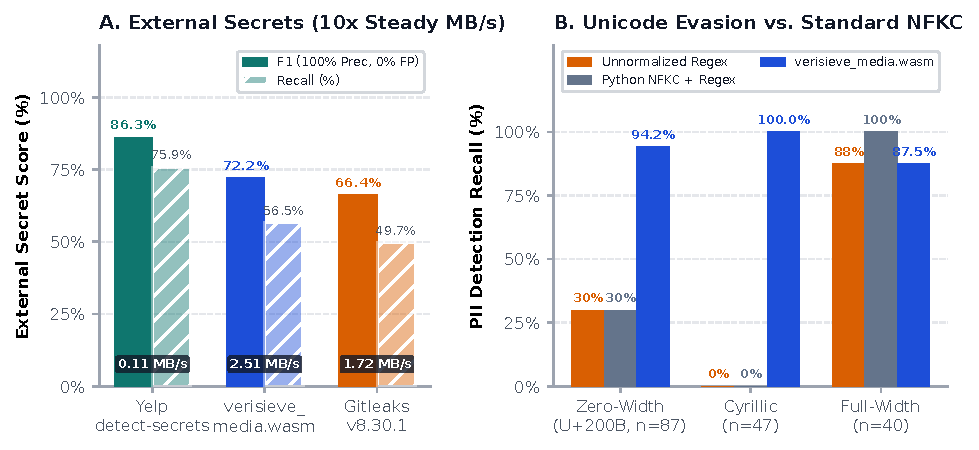
\includegraphics[width=0.98\textwidth]{figs/fig_e2_secrets_and_evasion.pdf}
\caption{\textbf{Exp.~3: Fair Steady-State Secret Scanning and Unicode NFKC Baseline.} (A)~Steady-state $10\times$ throughput (excluding process startup): \texttt{versieve\_media.wasm} sustains $2.51$\,MB/s ($\approx 1.5\times$ faster than \texttt{Gitleaks v8.30.1}, $22.8\times$ faster than \texttt{detect-secrets}) at $56.55\%$ recall / $72.25\%$ F1. (B)~Standard Python \texttt{NFKC} solves full-width digits ($100\%$) but still fails on zero-width spaces ($29.9\%$) and Cyrillic homoglyphs ($0.0\%$), where \texttt{versieve\_media.wasm} sustains $94.25\%$ and $100.0\%$.}
\label{fig:e2}
\end{figure*}

\subsection{Exp.~4: 25-Call End-to-End Audio PII Redaction with WASM \texttt{SR-MP} Phonetic Coupling}
\label{sec:exp4}

We synthesize $25$ realistic customer-service calls locally via offline Windows SAPI TTS ($97$ planted PII tokens across names, spoken emails, and spoken $10$-digit phones). The defender transcribes with \texttt{faster-whisper base.en} \citep{radford2023whisper} (word timestamps), runs \texttt{versieve\_media.wasm} Spoken ITN + Stage~3A/3B GLiNER-Edge, and silences matched spans ($60$\,ms padding, $5$\,ms cosine fade). We also evaluate \textbf{WASM \texttt{SR-MP} Phonetic-Coupled Audio Redaction}, which seeds the $512$-slot Salted Reference Sketch Ring \emph{only} from the engine's own in-call detections (Stage~3A/3B PERSON/EMAIL spans); a CI assertion holds that no scoring token can reach the seed arguments. The ring coalesces spoken-email connector tokens (\emph{``dot''}/\emph{``at''}) when \texttt{base.en} fuses or splits spoken addresses. Non-PII retention is a pre-declared word-recall count, not a claim that all non-PII speech survived: the benchmark declares $59$ non-PII context words across the $25$ calls and checks whether the attacker ASR (\texttt{small.en}) still recognizes each of them in the redacted audio. Four anchor-quality conditions complete the comparison: a plain Jaro-Winkler ($\ge 0.85$) baseline on the \emph{same} self-seeded anchor list, a wrong-record condition (ring seeded from a different call's detections), a partial-record condition (first anchor only), and a recall-ceiling analysis of planted tokens absent from every anchor. To avoid same-model bias, a \textbf{$3.3\times$ larger cross-model attacker} (\texttt{faster-whisper small.en}) evaluates raw and all redacted WAV conditions on the same planted-token denominator ($n{=}97$):
\begin{itemize}
    \item \textbf{Pre-Redaction Exposure:} $92/97 = \mathbf{94.85\%}$ (Wilson $95\%$ CI $[88.5\%, 97.8\%]$).
    \item \textbf{Isolated Spoken ITN + GLiNER Leakage:} $20/97 = \mathbf{20.62\%}$ (Wilson $95\%$ CI $[13.8\%, 29.7\%]$; $-74.23$\,pp drop, $15/25$ calls zero leak).
    \item \textbf{WASM \texttt{SR-MP} (self-seeded) Leakage:} $8/97 = \mathbf{8.25\%}$ (Wilson $95\%$ CI $[4.24\%, 15.44\%]$), an exact \textbf{$-86.60$\,pp absolute drop} ($91.30\%$ relative reduction of exposed tokens, $2.5\times$ lower residual leakage than isolated audio redaction, and \textbf{$21/25$ calls with zero residual leak}) while retaining \textbf{all $59$ pre-declared non-PII context words} under the attacker transcription (Figure~\ref{fig:e3}A).
    \item \textbf{Plain Jaro-Winkler Baseline (same anchors):} $7/97 = \mathbf{7.22\%}$ (Wilson $95\%$ CI $[3.54\%, 14.15\%]$; $22/25$ calls zero leak), marginally \emph{better} than the salted ring at matching.
    \item \textbf{Wrong-Record Anchors:} $19/97 = \mathbf{19.59\%}$ (Wilson $95\%$ CI $[12.9\%, 28.6\%]$); seeding the ring from a different call's record collapses the coupling gain back to the isolated baseline ($20.62\%$) without hurting non-PII retention (all $59$ words).
    \item \textbf{Partial-Record Anchors:} $16/97 = \mathbf{16.49\%}$ (Wilson $95\%$ CI $[10.4\%, 25.1\%]$); a partial record (first anchor only) roughly halves the coupling gain.
    \item \textbf{Recall Ceiling:} $27/97$ planted tokens never entered any anchor ($3.16$ anchors/call on average), and $7$ of the $8$ residual \texttt{SR-MP} leaks were among them; anchor-based coupling cannot recover what the detector never perceived.
\end{itemize}

\begin{figure*}[t]
\centering
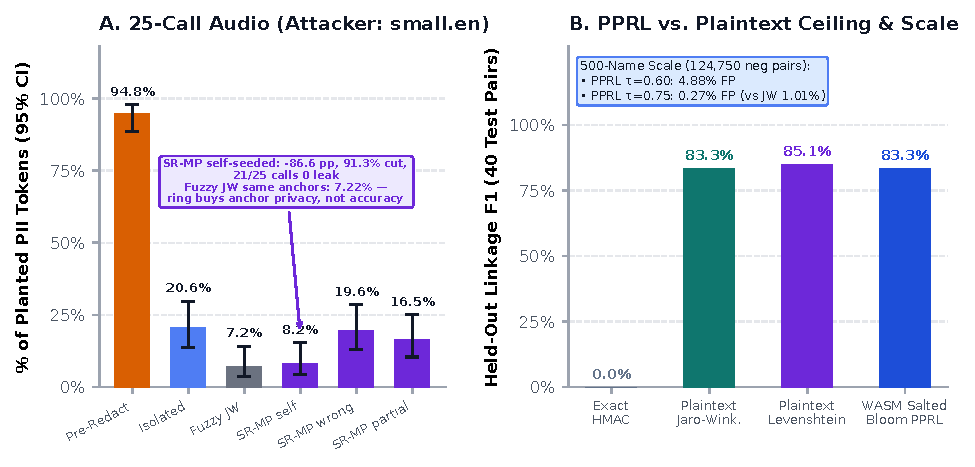
\includegraphics[width=0.98\textwidth]{figs/fig_e3_audio_e2e_and_pprl.pdf}
\caption{\textbf{Exp.~4 \& 5: Cross-Model Audio Redaction and PPRL Scale Reality Check.} (A)~$25$-call end-to-end audio benchmark evaluated by stronger cross-model attacker \texttt{faster-whisper small.en} on a single denominator ($n{=}97$ planted PII tokens, $95\%$ Wilson CIs): isolated Spoken ITN+GLiNER lowers exposure from $94.85\% \to 20.62\%$; self-seeded WASM \texttt{SR-MP} phonetic coupling cuts leakage to $\mathbf{8.25\%}$ ($-86.60$\,pp, $91.30\%$ relative reduction, $21/25$ calls zero leak) with all $59$ pre-declared non-PII context words retained; wrong-record/partial anchors collapse the coupling gain to $19.59\%$/$16.49\%$. (B)~On $40$ held-out noisy pairs (threshold tuned strictly on disjoint dev), zero-import salted Bloom+Soundex PPRL matches plaintext Jaro-Winkler ($83.33\%$ F1); across $124{,}750$ common-name negative pairs, tightening $\tau$ from $0.60 \to 0.75$ cuts pairwise false links from $4.88\%$ to $0.27\%$ (vs.\ $1.01\%$ for plaintext Jaro-Winkler).}
\label{fig:e3}
\end{figure*}

\subsection{Exp.~5: PPRL Reality Check, \texttt{SR-MP} Ring Architecture, and Kernel Sanity}
\label{sec:exp5}

To avoid overfitting small hand-crafted pairs, we tune thresholds strictly on a disjoint $20$-pair Dev set ($\tau_{\text{Dice}}{=}0.60$) and evaluate on $40$ held-out Test pairs ($20$ OCR/ASR noisy + $20$ hard same-first-name negatives) against \textbf{plaintext non-private ceilings} (Jaro-Winkler and normalized Levenshtein). On held-out Test, Exact HMAC scores $0.0\%$ F1, Plaintext Levenshtein reaches $85.11\%$ F1 ($74.1\%$ P / $100\%$ R), Plaintext Jaro-Winkler reaches $83.33\%$ F1 ($71.4\%$ P / $100\%$ R), and zero-import WASM Salted Bloom+Soundex PPRL matches Jaro-Winkler at \textbf{$83.33\%$ F1} ($71.4\%$ P / $100\%$ R) (Figure~\ref{fig:e3}B).

\paragraph{Scale Collision Test ($500$ Common Names $= 124{,}750$ Negative Pairs).}
Evaluating all $500 \times 499 / 2 = 124{,}750$ distinct full-name pairs ($25$ common first $\times$ $20$ common last names) demonstrates why permissive thresholds cannot be deployed at scale: at $\tau{=}0.60$, pairwise false links reach \textbf{$4.88\%$ ($6{,}090/124{,}750$)}, whereas tightening to $\tau{=}0.75$ lowers false links $18\times$ to \textbf{$0.270\%$ ($337/124{,}750$)}, $3.7\times$ fewer collisions than Plaintext Jaro-Winkler ($1.007\%$, $1{,}256/124{,}750$). Furthermore, we explicitly caution against over-claiming cryptographic privacy for $128$-bit Bloom filters: small Bloom encodings are vulnerable to frequency-analysis cryptanalysis when an attacker has auxiliary population lists \citep{christen2018bloomattack}, and Soundex is English-centric; thus PPRL in Versieve-MM should be treated as a \emph{local-only noisy erasure index}, never a safe external export format.

\paragraph{Sparse-Reference Multimodal Perception (\texttt{SR-MP}) \& \texttt{GC-CRC} in $O(1)$ WASM Memory.}
To resolve the \emph{fragmented context horizon} of chunk-isolated detectors in $O(1)$ bounded memory (inspired by sparse reference pools in long-horizon document perception), we compile a static $512$-slot ($16$\,KB, $32$\,B/slot) \textbf{Salted Reference Sketch Ring} directly into \texttt{versieve\_media.wasm} (\texttt{vs\_media\_srmp\_reset}, \texttt{vs\_media\_srmp\_seed\_anchor}, \texttt{vs\_media\_srmp\_query\_candidate}) and wire it into \texttt{src/perceive.js} (\texttt{GC-CRC} / \texttt{SR-MP}). Each slot stores a $128$-bit salted 2-gram Bloom filter (\texttt{u64} pair), a $64$-bit salted Soundex hash, a $32$-bit exact token FNV-1a hash, and $8$\,B of metadata (\texttt{entity\_uid}, \texttt{block\_idx}, \texttt{conf\_x1000}, \texttt{popcount}, \texttt{canon\_len}, \texttt{kind\_code}), propagating anchor risk across document paragraphs, presentation slides, audio ASR turns, and video OCR keyframes via:
\begin{equation}
\resizebox{\columnwidth}{!}{$S_{\text{SR-MP}}(m, c) = 1 - \bigl(1 - s_{\text{local}}(m)\bigr)\bigl(1 - \gamma \max_{a \in \mathcal{R}_{512}} \operatorname{Sim}(\text{sig}(m), \text{sig}_a)(1 + \beta d_{a,c}^{-1})\bigr).$}
\end{equation}
Beyond its real-benchmark gains on TAB ECHR rulings (Table~\ref{tab:tab-bench}) and $25$-call Whisper audio (Figure~\ref{fig:e3}A), across a $60$-case, $240$-block ($4$-modality) cross-modal stress suite (\texttt{scripts/eval-gccrc-benchmark.mjs}), isolated high-precision hybrid filtering ($\tau{=}0.60$) misses $100\%$ of weak cross-modal follow-ups ($44.64\%$ F1), while lowering the isolated threshold to $\tau{=}0.20$ inflates domain false positives by $+140\%$ ($75 \to 180$ FPs). By contrast, \textbf{WASM \texttt{SR-MP} / \texttt{GC-CRC}} ($\tau_{\text{anchor}}{=}0.60$) recovers \textbf{$76.11\%$} of noisy cross-modal follow-ups ($83.03\%$ consistent entity-link rate) with \textbf{zero} extra domain false positives ($75$ FPs, \textbf{$77.74\%$ precision}, \textbf{$75.18\%$ F1}).

Finally, Table~\ref{tab:micro} records compact kernel micro-benchmarks separately from accuracy comparisons.

\begin{table}[t]
\caption{Compact kernel micro-benchmarks (systems sanity metrics, distinct from competitive accuracy benchmarks).}
\label{tab:micro}
\vskip 0.08in
\begin{center}
\resizebox{\columnwidth}{!}{%
\begin{tabular}{llr}
\toprule
\textbf{Kernel Subsystem} & \textbf{Verified Operation} & \textbf{Measured} \\
\midrule
Forensic Scrub ($7/7$ caught) & JPEG EXIF, EML, HAR, DOCX \texttt{delText}, K8s, PPTX, XLSX & $0.009$--$0.162$\,ms \\
Enron Email Ingestion & $500$ \texttt{Yale-LILY/aeslc} \citep{zhang2019aeslc} emails ($2{,}769$ PII spans) & $3{,}399$ emails/s \\
Archive Bomb Defense & $64$\,MB ZIP-bomb ($1{,}026\times$ ratio) mid-stream abort & $0.521$\,ms \\
Graph GDPR Blast Radius & $5{,}000$ blocks / $20{,}200$ edges ($5$ modalities, WASM) & $0.915$\,ms \\
\bottomrule
\end{tabular}%
}
\end{center}
\vskip -0.14in
\end{table}

\section{Limitations and Operating Boundaries}
\label{sec:limitations}

\begin{enumerate}
    \item \textbf{Edge vs.\ Server NER Gap:} On TAB legal rulings, Microsoft Presidio (\texttt{en\_core\_web\_lg} + ECHR code regex, $400.7$\,MB) outperforms our $45.8$\,MB edge GLiNER pipeline by $+33.35$\,F1 on All-Maskable entities ($79.26\%$ vs.\ the Hybrid edge system's $45.91\%$) and by $+12.07$\,F1 on \texttt{PERSON} ($86.27\%$ vs.\ Dev-Filtered GLiNER's $74.20\%$), and adding $45.8$\,MB GLiNER to Stage~3A+Code lowers All-Maskable F1 ($51.67\% \to 45.91\%$).
    \item \textbf{Modest Overall Gate Automation, Heuristic Cluster Correction \& Detector-Closed Scope:} On PII-dense TAB rulings ($81.2\%$ unsafe, $\operatorname{DEFF}{=}2.62$), Document-Clustered \texttt{HC-CRC} removes the $\alpha{=}0.10$ FPR overshoot ($8.19\% \le 10\%$, $18.91\%$ overall auto-release) and certifies $2.53\% \le 5\%$ at $\alpha{=}0.05$ ($9.55\%$ auto-release) as well as $0.18\% \le 1\%$ at $\alpha{=}0.01$; its cluster-robustness rests on a survey-sampling design-effect heuristic compared directly against guarantee-backed Dunn, Lee, and \texttt{HG-CRC} baselines in Sec.~\ref{sec:exp2} (Table~\ref{tab:hier-baselines}), where all formal cluster bounds fail closed at $\alpha{=}0.01$ under $M_0{=}67$ and streaming \texttt{E-LTT} fails closed at $\alpha \le 0.02$ ($E_{\max}{=}1$, zero auto-release). Moreover, because scrubbed text can still leak private attributes to inference attacks \citep{lukas2023pii,staab2024beyond}, detector-closed gating must be paired with adversary-aware auditing \citep{cpa2026auditing} when quasi-identifier singling-out is in scope.
    \item \textbf{Audio, Secrets, and PPRL Scope:} Exp.~4 uses locally synthesized TTS audio ($25$ calls in clean synthetic speech; $8.25\%$ residual leakage under self-seeded \texttt{SR-MP} vs.\ $20.62\%$ isolated, under \texttt{small.en}) rather than noisy telephony speech; Exp.~3 uses short \texttt{MBPP} scripts and synthetic external credentials; and $128$-bit Bloom+Soundex PPRL is English-centric and vulnerable to frequency attacks if exported externally \citep{christen2018bloomattack}.
    \item \textbf{Portable Runtime Split:} Stage~3A WASM (secrets, anti-evasion, containers, PPRL, \texttt{SR-MP} ring, WAV/canvas redaction) runs live in the RTIO browser sandbox today, while Stage~3B ONNX GLiNER and local Whisper ASR currently execute in Node/Python and fail closed without local weights; OCR on dark stylized slides also benefits from modern ONNX OCR \citep{cui2025paddleocr,ibm2025granitedocling}.
\end{enumerate}

\section{Conclusion}
\label{sec:conclusion}

Versieve-MM demonstrates a verifiable zero-import WebAssembly systems architecture ($204{,}031$\,B, $29$ exports, $0$ host imports) spanning enterprise container auditing, $2.51$\,MB/s steady-state secret scanning, $O(1)$ Sparse-Reference Multimodal Perception (\texttt{SR-MP}), client-side audio/visual redaction, and noisy cross-modal erasure. Evaluation against strong third-party baselines confirms that compact $45.8$\,MB edge NER models still trail $400$\,MB server pipelines like Presidio on out-of-distribution legal text, while WASM \texttt{SR-MP} anchor coupling ($88.41\%$ TAB Person recall; $8.25\%$ vs.\ $20.62\%$ cross-model Whisper audio leakage) and Document-Clustered Conformal Risk Control (\texttt{HC-CRC}, $0.18\%$--$8.19\%$ Conditional FPR across $\alpha \in [0.01, 0.10]$) provide a conservative, fail-closed perception and release layer under local-only constraints that prohibit server-side stacks.

\bibliography{versieve-multimodal-sanitization-benchmark}
\bibliographystyle{mlsys2025}

\appendix
\section{Zero-Import WASM Audit and Verification Surface}
\label{app:audit}

All five Versieve WebAssembly modules enforce \texttt{imports.length === 0} at load time (Table~\ref{tab:wasm-audit}), and the local MCP server exposes $18$ tools, verified by the local test suite (Node.js CI $220$ tests across $38$ files, Rust unit $6/6$, Python $4/4$, RTIO Next.js build + browser unit tests $9/9$).

\begin{table}[h]
\caption{Load-time zero-import audit across all five Versieve WebAssembly modules.}
\label{tab:wasm-audit}
\vskip 0.08in
\begin{center}
\resizebox{\columnwidth}{!}{%
\begin{tabular}{lrr>{\raggedright\arraybackslash}p{1.45in}}
\toprule
\textbf{WASM Binary} & \textbf{Bytes} & \textbf{Imports} & \textbf{Primary Role} \\
\midrule
\texttt{versieve\_clean.wasm} & $14{,}633$ & $0$ & Normalization, dedupe, chunking \\
\texttt{versieve\_sql.wasm} & $55{,}635$ & $0$ & Local SQL filtering, inner equi-join \\
\texttt{versieve\_graph.wasm} & $54{,}402$ & $0$ & Dual-CSR graph, PPR, GDPR blast \\
\texttt{versieve\_dl.wasm} & $60{,}096$ & $0$ & BitNet, VeRA, 64-d retrieval \\
\texttt{versieve\_media.wasm} & $204{,}031$ & $0$ & Archives, secrets, PPRL, \texttt{SR-MP}, ITN, media \\
\bottomrule
\end{tabular}%
}
\end{center}
\vskip -0.10in
\end{table}

\end{document}
